    \documentclass{article}

% if you need to pass options to natbib, use, e.g.:
%     \PassOptionsToPackage{numbers, compress}{natbib}
% before loading neurips_2019

% ready for submission
% \usepackage{neurips_2019}

% to compile a preprint version, e.g., for submission to arXiv, add add the
% [preprint] option:
%     \usepackage[preprint]{neurips_2019}

% to compile a camera-ready version, add the [final] option, e.g.:
\usepackage[]{neurips_2019}

% to avoid loading the natbib package, add option nonatbib:
%     \usepackage[nonatbib]{neurips_2019}

\usepackage[utf8]{inputenc} % allow utf-8 input
\usepackage[T1]{fontenc}    % use 8-bit T1 fonts
\usepackage{hyperref}       % hyperlinks
\usepackage{url}            % simple URL typesetting
\usepackage{booktabs}       % professional-quality tables
\usepackage{amsfonts}       % blackboard math symbols
\usepackage{nicefrac}       % compact symbols for 1/2, etc.
\usepackage{microtype}      % microtypography
\usepackage{authblk}
\usepackage{graphicx}
\title{News Recommendation Engine}

\author[1]{Ankita Pal\thanks{A.apal1994@uw.edu}}
\author[1]{Chavi Gupta\thanks{B.chavig@uw.edu}}
\author[1]{Medha Sagar\thanks{C.sagarme@uw.edu}}
\affil[1]{Department of Data Science, University of Washington}

\renewcommand\Authands{ and }

\begin{document}
\maketitle

\begin{abstract}
    The goal of this project is to build a News Recommender System. We chose to work on a News Recommender system since we were interested in addressing both the dimensionality (associated with large text content) and recommendation problems that were covered in class. Among the different domains of recommender systems, news recommendation has been explored relatively less due to the lack of structured data and features. Text mining for news articles using NLP techniques in itself is a different class of problem. In this project we aim to build a pipeline for extracting user and news article features, and eventually build a hybrid recommender system to address the problems of cold start, data sparcity and scalability. 
\end{abstract}

\section{Reaction Paper}

\subsection{Hybrid Recommender Systems: A Systematic Literature Review}
\href{https://arxiv.org/pdf/1901.03888.pdf}{Link to paper}

\subsubsection{Summary}
For choosing an algorithm for our news recommendation system, we analyzed the problem and found that there were some basic challenges that we could face while using the traditional Collaborative Filtering or Content-based Filtering techniques that were discussed in class. They included the cold start problem (in terms of both new users and new news articles). There was also the issue of very sparse data since the vast universe of articles and users on twitter is tremendous. Thus we decided that we needed to use a hybrid approach.
This is how we came across this detailed Literature Review on different Hybrid Recommender Systems \cite{litReview}. This literature review was done based on surveying around 76 papers from various digital journal sources. Since the paper is relatively recent (2017), we believe that the trends and findings are quite up to date. This literature review was extremely helpful since it analyzed core questions like:

\begin{enumerate}
    \item What type of research problems (e.g. cold start, data sparsity, accuracy, scalability, etc.) were addressed by different papers and algorithms,
    \item Which are the most common Data mining and ML techniques used to build hybrid recommender systems,
    \item What are the most common combinations in Hybrid RecSys,
    \item What are the techniques to combine the algorithms in a hybrid system,
    \item What are the evaluation techniques generally used for hybrid recommender systems
\end{enumerate}

\subsubsection{Critique}
Each of these questions was answered for us with references to other research papers that showed different problem characteristics. By comparing our proposed problem against other problems, we were able to gather a lot of insight into the approach we would like to take for our hybrid algorithm.  Some of the drawbacks of this paper were in the lack of technical details and mathematical formulations regarding the different approaches and algorithms. Another shortcoming is that although the paper uncovers trends, it does not delve into the causes or the explanations behind why these trends were discovered or why a particular research problem is usually targeted in a particular way.
Overall the paper was quite easy to read through and gives a lot of direction into Hybrid Recommendation Systems. By brainstorming on the above questions we began to build a pipeline for our recommender system.

\subsubsection{Brainstorming}
We found that one of the most common approaches for the cold start and sparsity issues is the CF-CBF approach. The problem can then be further broken down into the subtasks of creating user profiles, news article profiles, an interaction matrix and eventually a recommender system that can put it all together.
Based on the survey, KNN and Clustering are the most general techniques used to create profiles. Clustering techniques for profile creation handles the problem of cold start and scalability (dimensionality reduction) quite well. Thus we decided to explore more into the use of a clustering algorithm for user profile creation.
Since the articles are text based data, we require some text mining strategies to profile the data. We explored different techniques and found that TF-IDF, SVD and LDA were the most common techniques for creating feature representations of the data. 


\subsection{Scalable news recommendation using multi-dimensional similarity and Jaccard–Kmeans clustering}
\href{https://www-sciencedirect-com.offcampus.lib.washington.edu/science/article/pii/S0164121214001162}{Link to paper}

\subsubsection{Summary}
Main technical content of the paper revolves around making a scalable news recommendation using multi-dimensional similarity and Jaccard–Kmeans clustering. The paper is related to the topics presented in the course. The Jaccard similarity and K-means clustering were part of our course syllabus. The paper tries and combines the two and helps build a more scalable news recommender. 

\subsubsection{Critique}
The paper takes into consideration all the aspects of the news recommendation – the user behavior, the type of content, and the time of accessing the news. It also explains the impact of each factor on accuracy of the recommender. 

The paper does not given in-depth understanding of the maths behind the basic algorithms. The author expects the user to know the maths behind the LSH and K-means clustering. This may be confusing for a person new to this area. A proper description of the dataset. Some key statistics of the datset were give, but details of the columns and their description was not provided along with the paper.Also, For the Top N recommendations the paper assumes for a user, if a neighbour accesses a piece of news at a time closer to the present time, the more will be the probability that the user will access the news. Thus, the time of access will greatly influence the recommendation to a user. This may not always be true. For example, if the neighbor has to mistakenly access an article. It may have been used very recently, but it is not relevant to the user or the neighbor .

The proofs in the paper seem technically sound. The author has well explained the logic for each step he has taken and the calculation or formula he has used.The theorems are easy to understand. They convey the meaning that the authors have claimed.

\subsubsection{Brainstorming}
A promising further research would be to take into consideration the amount of time the user and neighbor spent on the news previously if accessed. This may help us remove mistaken access to the news. This would refine the clustering data.The paper dismisses the effects of the demographics of the users. Adding to the assumption list that there would be an effect of demographics would be an interesting study.This addition would require additional data for the demographics of the users. Also, the similarity in terms of demographics would be needed to be calculated to incorporate into the model

\subsection{Latent Dirichlet Allocation}
\href{http://www.jmlr.org/papers/volume3/blei03a/blei03a.pdf2}{Link to Paper}

\subsubsection{Summary}
The given paper discusses a probabilistic text modelling technique called \textbf{Latent Dirichlet Allocation} which addresses the problem of modelling text corpora and other discrete data collections. 

The goal of the research is to find short descriptions of documents in large corpora in an efficient manner that preserves the statistical relationship between the documents and the corpora. We call this process \textbf{Topic Modelling}.

In our course we have studied Singular Value Decomposition (SVD) for dimensionality reduction. There are some techniques such as, LSA (Latent Semantic Analysis) which utilize the concept of SVD to minimize the dimensions before classifying topics in documents. Additionally, we studied about TF-IDF technique that reduces documents with varying lengths to fixed size lists representations. 

The shortcoming of the above two techniques is the same, while these methods are efficient in reducing the dimensions and extracting features, they do not possess any generative probabilistic nature to model language. So, assigning probabilities to documents not in the training set is a major challenge. Also, both the techniques are based on the "bag-of-word" approach, and do not take into account the order of the words in the documents. 

These shortcomings are addressed by the Latent Dirichlet Allocation algorithm proposed in the paper. 

\subsubsection{Critique}

The paper discussed in this section takes into account generative probabilistic model of a corpus. The model has two aggregation layers. The first layer assumes that the documents are represented as random mixtures over topics, and the second aggregation layer assumes that each topic is characterized by distribution over words. 

By combining the two layers we can effectively model large corpus containing documents and classify documents into categories and also achieve a level of summarization. 

The assumptions made by the authors are simple. The first assumption is that the number of topics are fixed. Secondly, all the documents are generated by a generative process and the topics are distributed over a fixed vocabulary.

The equations described in the paper requires understanding of certain probability distributions. The proofs presented in the paper are explained well and are easy to follow. The proofs are followed by experiments that address different application of the algorithm. 

In the first experiment, LDA was used to model documents and its performance was measured along with other techniques such as pLSI (probabilistic latent semantic indexing) and the unigram model. The experiments show that both pLSI and the unigram model suffer from over-fitting but due to different reasons. While the unigram model leads to deterministic clustering of the training documents, which make it harder to estimate the likelihood of new words in the test data set, pLSI model shows overfitting because of the dimensionality of one of its parameters and the assumption that one document can contain different proportions of topics. 

The second experiment explains the use of LDA in document classification. In this experiment, LDA was used as dimensionality reduction technique. In particular, LDA reduces any document to a fixed set of real-valued features associated with the document. 
Two classifiers were trained - one using LDA features and the other using all word features.
The conclusion was that LDA was able to reduce the feature vector space by 99.6\% with very little reduction in the classification accuracy. 

\subsubsection{Brainstorming}

We see a great potential in using LDA for creating feature vector space on news articles. The only hurdle we might face would be estimating the news categories. But we can use some other unsupervised technique to find optimal news clusters or categories.

After exploring the profiling techniques, we will use a hybrid approach to generate recommendations based on both content based and collaborative-filtering approaches. For this we found multiple papers that suggested complex approaches to combine the algorithms. We also found a popular algorithm called LightFM \cite{lightfm} that has been implemented as a Python library. However since we were interested in implementing our own technique, we would like to come up with a simpler way to do this. One possible way we propose is by using the similarities between the user groups and the news articles to recommend news articles to users that are within a user group. This approach will be developed upon as we proceed further in the project.

\section{Project proposal}
\label{gen_inst}

Finally to reiterate on the problem statement, the goal is to build a recommendation engine that can recommend news articles to users based on their past history and interests as well as based on what other users like them have viewed. This is very useful for blogging and news platforms that would like to attract users to continue viewing more articles within the platform. By recommending relevant articles that a user would view, these platforms can maintain user engagement and prevent users from exiting out and viewing other platforms. It also reduces the number of search queries that a user may have to do to find more articles. All in all, it’s a win-win for both the users and the news platforms. Eventually, the objective is to be able to recommend articles that a user is most likely to view next.

\subsection{Proposed Data Source}
For a hybrid recommendation system, we require data for both user and news article profiling. We decided to use the web scraping tool by the authors of the FakeNewsNet paper \cite{datasrc} that collects data for various twitter users and pulls text content from different news article urls. While the data is split as fake news and real news, our objective is not to classify the news articles as fake or real. However, we do intend to utilize the rich collection of data that is gathered by the tool. The tool also has an advantage of choosing a domain for the news articles and the features that we want to download. 

The news recommendation engine has many facets and subproblems associated with it. We have divided the entire problem into sub-parts and have strived to come up with different techniques that might address these problems. 
The following table summarizes some of the problems and our proposed solutions. 
User-Side Cold Start Problem
In order to be able to recommend articles to new users, we will be using hierarchical clustering to segment users into groups  
Item-Side Cold Start Problem
News Articles that are new and have very less metadata associated with them will be modelled using Latent Dirichlet Allocation to find out 


\subsection{Proposed Approach}
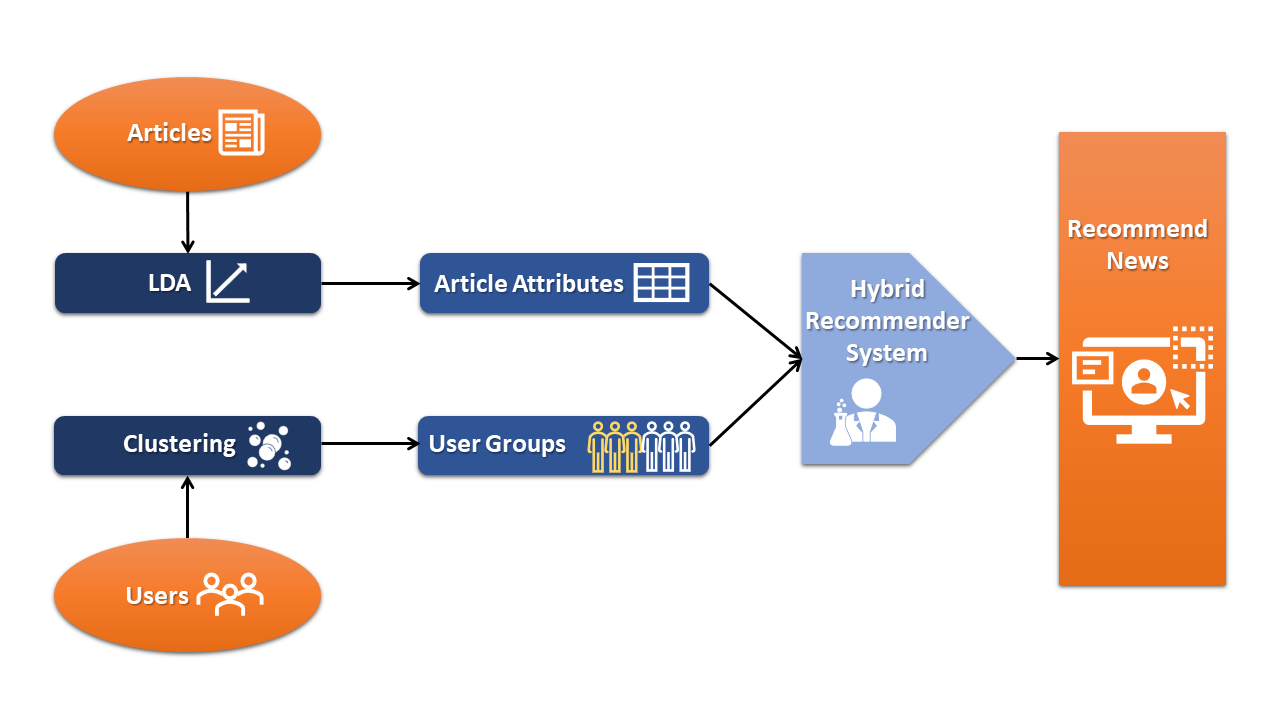
\includegraphics[scale=.50]{NeuRIPS2019/Slide1.PNG}

\begin{thebibliography}{9}

\bibitem{litReview} Çano, E.,\& Morisio, M.\ (2017). Hybrid recommender systems: A systematic literature review. {\it Intelligent Data Analysis}, 21(6), 1487-1524.

\bibitem{lightfm} Kula, M. (2015). Metadata embeddings for user and item cold-start recommendations. {\it arXiv preprint arXiv:1507.08439}.
Bower, J.M.\ \& Beeman, D.\ (1995) {\it The Book of GENESIS: Exploring
  Realistic Neural Models with the GEneral NEural SImulation System.}  New York:
TELOS/Springer--Verlag.

\bibitem{datasrc} Shu, K., Mahudeswaran, D., Wang, S., Lee, D.,\ \& Liu, H. (2018). FakeNewsNet: A Data Repository with News Content, Social Context and Spatialtemporal Information for Studying Fake News on Social Media. {\it arXiv preprint arXiv:1809.01286}.

\end{thebibliography}
\end{document}
